\section{Simulation results} 
To make the simulation results easier to understand we begin by outlining a baseline model with one independent variable of interest and two covariates split by the different model sets. we then show the results of what happens when including more covariates, what happens when the sample size increases or decreases, and having different correlations between the dependent variable and covariates. 

\subsection{Model specification}
Looking at the FPP and FPR between the different sets in the baseline model, it is clear that the highest FPP and FPR are obtained in the $x \times z$ and $x + z+ x \times z$ sets (see Figure \ref{fig:mainfigure1}). This is the case when using interaction effects both when the corresponding main effects are present and whey they are not present. When the corresponding main effects are not present and the variable of interest and covariates are binary and dummy coded, the FPP and FPR are particularly high. This is because the dummy coded variable of interest splits the true effect of the covariate into the interaction and the constant. In this case, the FPP for the $x \times z$ set is 82.7\% and 86.9\% for the $x + z+ x \times z$ set. When the variables are continuous and everything else is equal, the FPP for the two sets are 18.8\% and 23.5\%, respectively. With the restriction that main effects must follow interactions, only the $x + z+ x \times z$ set remains because the $x \times z$ set becomes an empty set. In this case, the FPP is 21.1\% for binary (dummy coded) variables and 18.1\% for continuous variables. \\ 
Looking at the FPR, we see that in many model sets the proportion of models with a significant effect is around the expected 5\%  (see red bars in Figure \ref{fig:mainfigure1}). However, in sets with interactions between the variable of interest and covariates with omitted main effects (left hand side of Figure \ref{fig:mainfigure1}), the FPR is above 5\%. For the $x \times z$ set with binary and dummy coded variables and without corresponding main effects the FPR is 34.5\%.
 \\

% plot of main analysis
\begin{figure}[hbt!]
%\figuretitle{Baseline model}
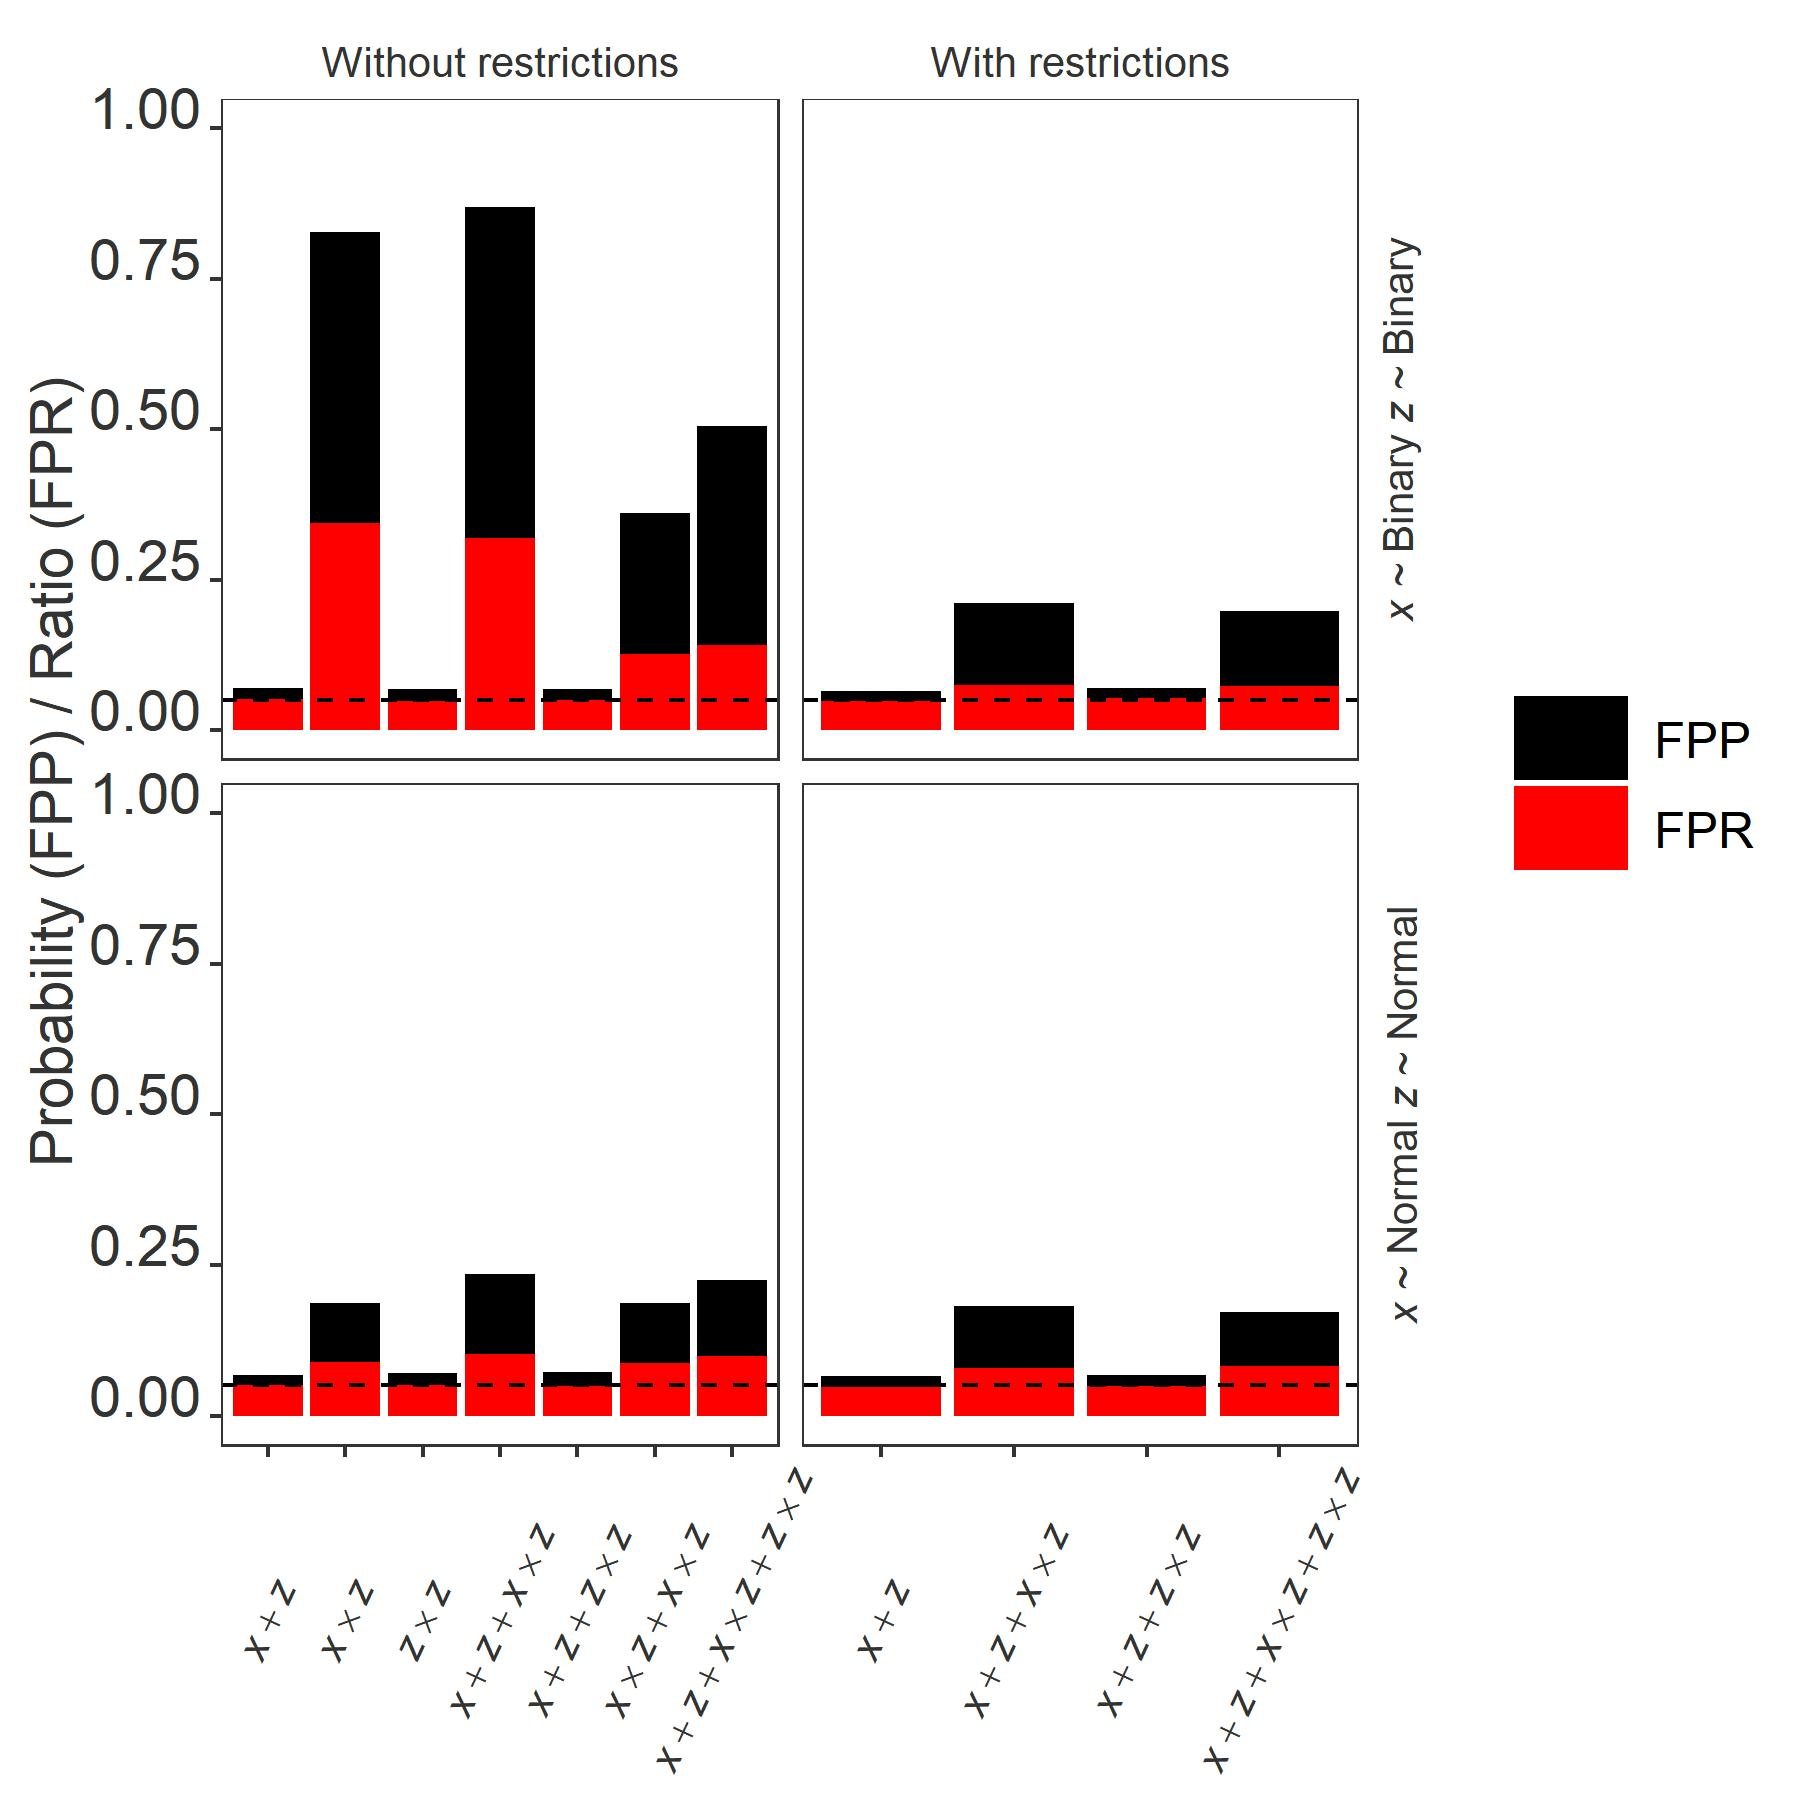
\includegraphics[width=0.6\textwidth]{R/Analysis/Result/Figures/Figure1A.jpeg}
\centering
\caption{The false-positive probability and false-positive ratio given different model sets, the presence of main effects when having interactions, and different distributions of the variable of interest and covariates. Sample size is set to 200, the correlation between the dependent variable and covariates is $r=0.2$, and there are two covariates. The false-positive probability is shown in black and the false-positive ratio in red. Dashed blacked line shows the critical value, here set at 0.05 }.
\label{fig:mainfigure1}
\end{figure}

\subsection{Number of covariates}
Adding one more covariate to the baseline model to get three in total increases the FPP across all model sets (see Figure \ref{fig:mainfigure2}). The increase is the highest for binary and dummy coded variables with no restrictions on main effects to follow interaction effects. Several of the sets with interactions between the variable of interest and covariates reach an FPP of just below 100\%. The increase is also evident even when main effects are present when having interactions. In that case, the largest increase in the FPP is in the $x + z+ x \times z + z \times z$ set which increases 14.7 percentage points when the variable of interest and covariates are binary (dummy coded) and 13.1 percentage points when the variables are continuous. The FPR also increases for all sets with an interaction between the variable of interest and covariates although the main increase happens when there is no restriction that main effects most follow interactions and when the variables are binary and dummy coded.

% plot of main analysis
\begin{figure}[hbt!]
%\figuretitle{Effect of increasing the number of covariates}
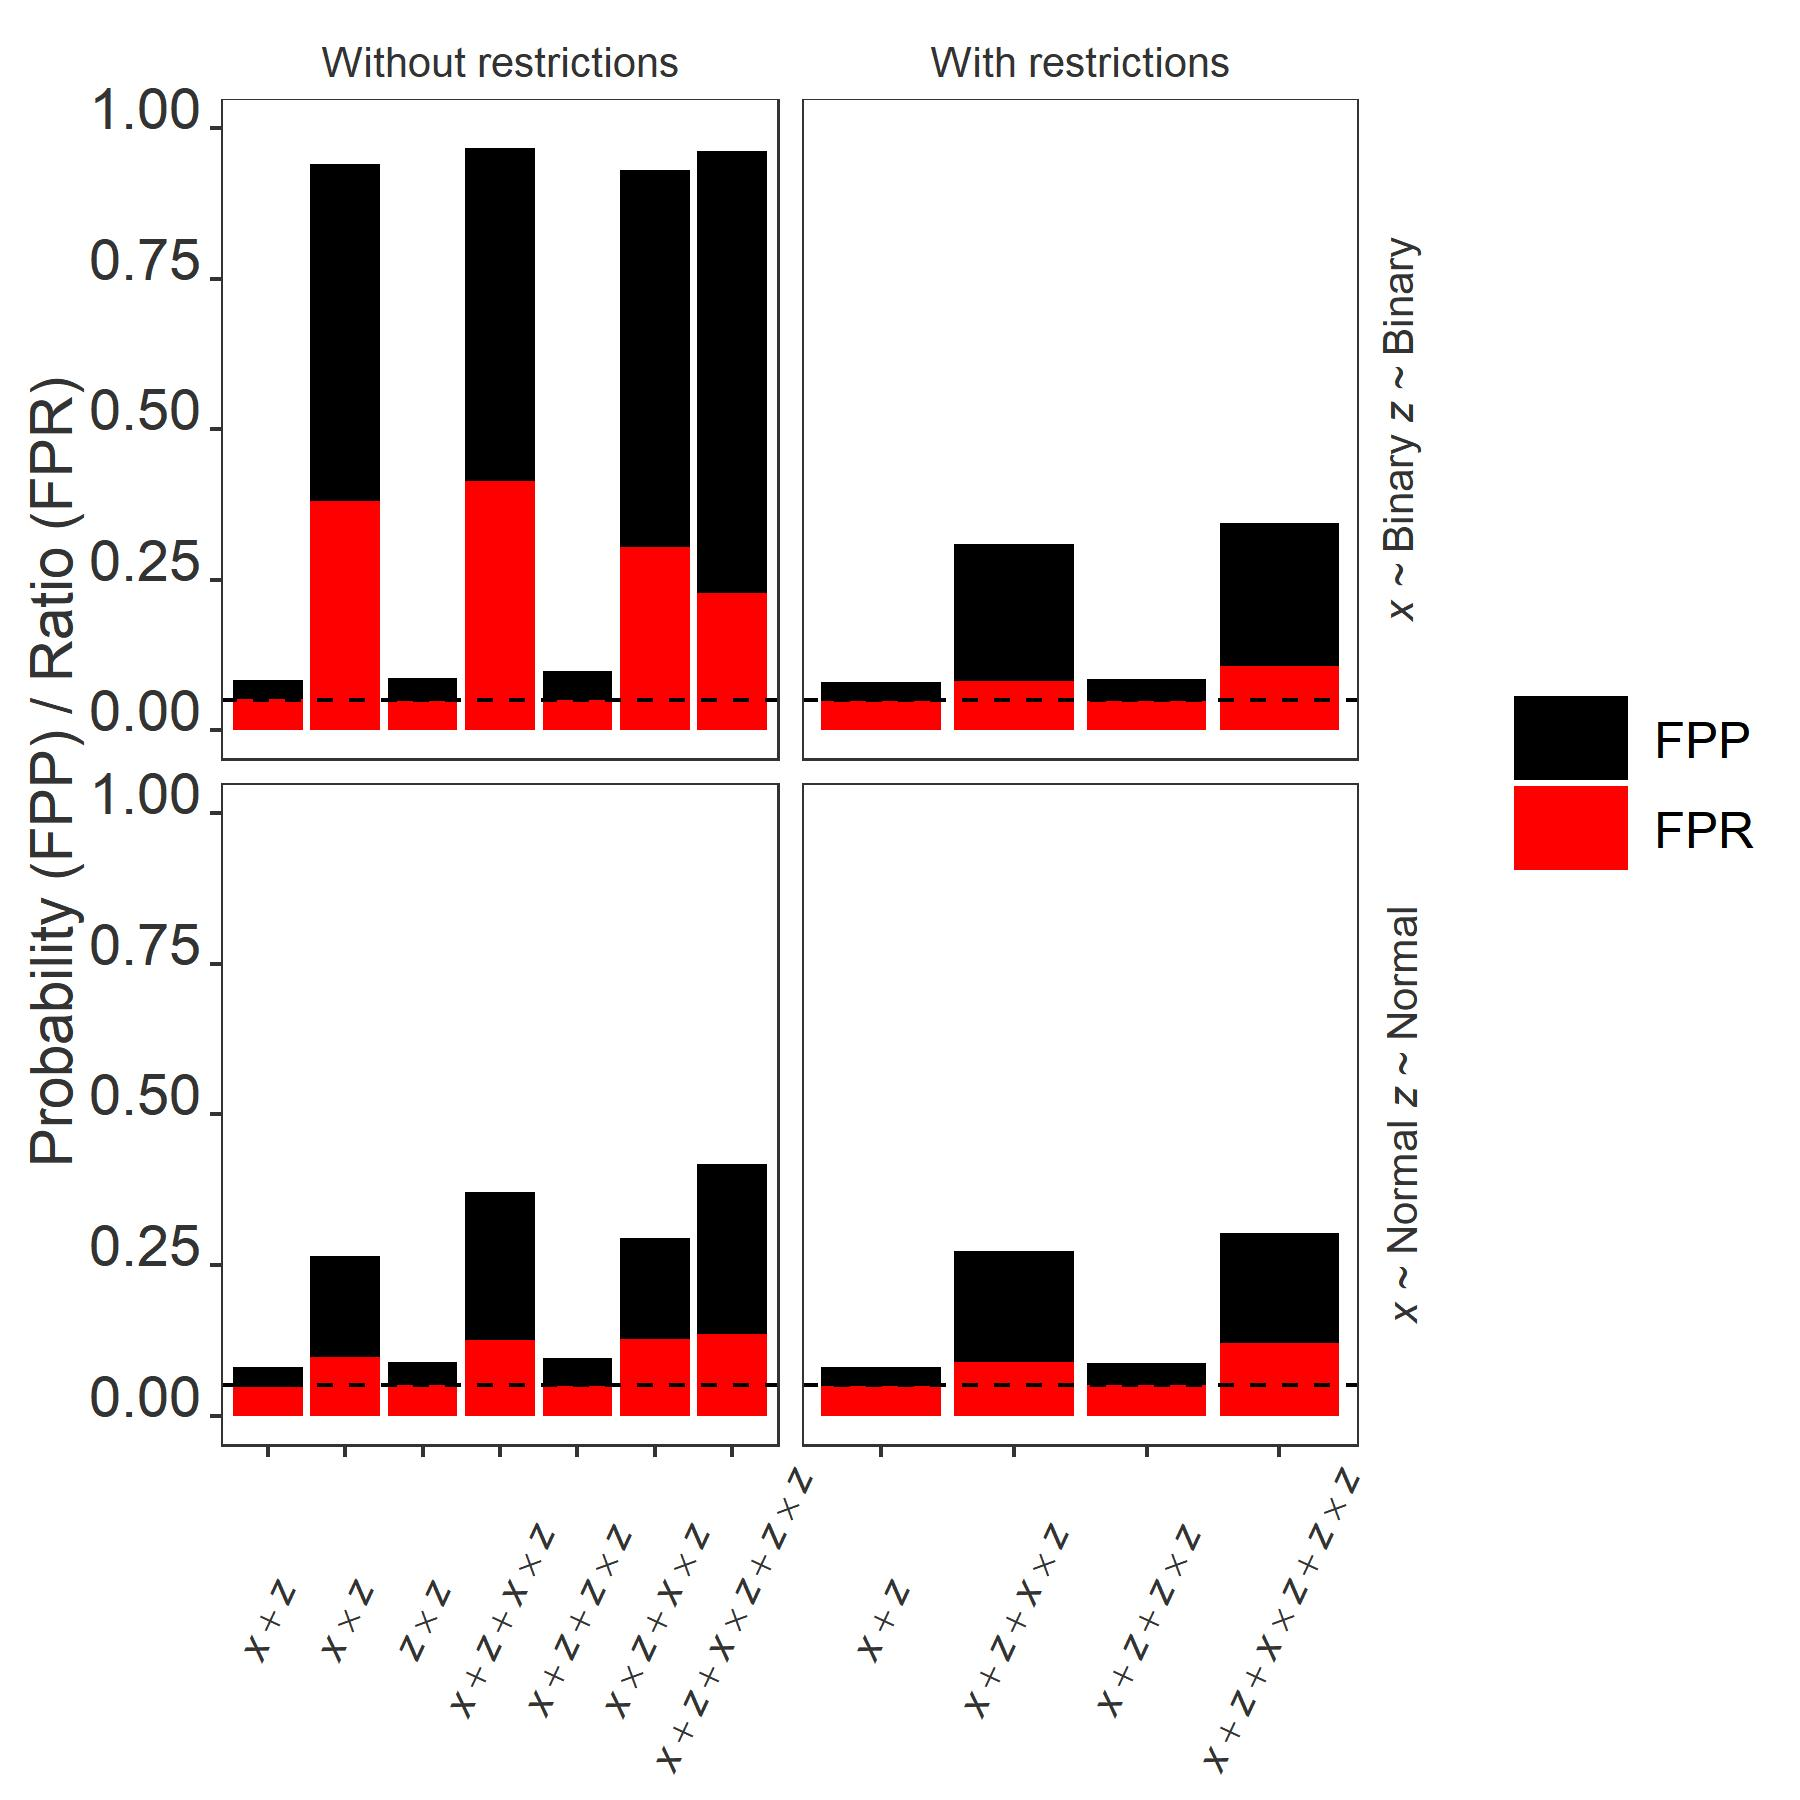
\includegraphics[width=0.6\textwidth]{R/Analysis/Result/Figures/Figure1C.jpeg}
\centering
\caption{The false-positive probability and false-positive ratio when using three covariates. Black bars are the false-positive probability and red denotes the false-positive ratio. Dashed blacked line shows the critical value, here set at 0.05. The description of the figure is otherwise the same as for Figure \ref{fig:mainfigure1}.}
\label{fig:mainfigure2}
\end{figure}

\subsection{Sample size}
Increasing the sample size in the baseline model and thereby improving the precision of the estimates has, in most of the conditions, no effect on either the FPP or FPR. However, in sets with interactions between the variable of interest and covariates where main effects are not included and variables are binary and dummy coded, larger sample sizes increase the FPP (See Figure \ref{fig:mainfigure4}). In the $x \times z$ and $x + z+ x \times z$ sets the FPP reaches just below 100\% as the sample size increases to 300. In these sets, the larger sample sizes also lead to increases in the FPR with the largest increase of 41.9\% for the $x \times z$ set.  


\begin{figure}[hbt!]
%\figuretitle{Effect of increasing the sample size}
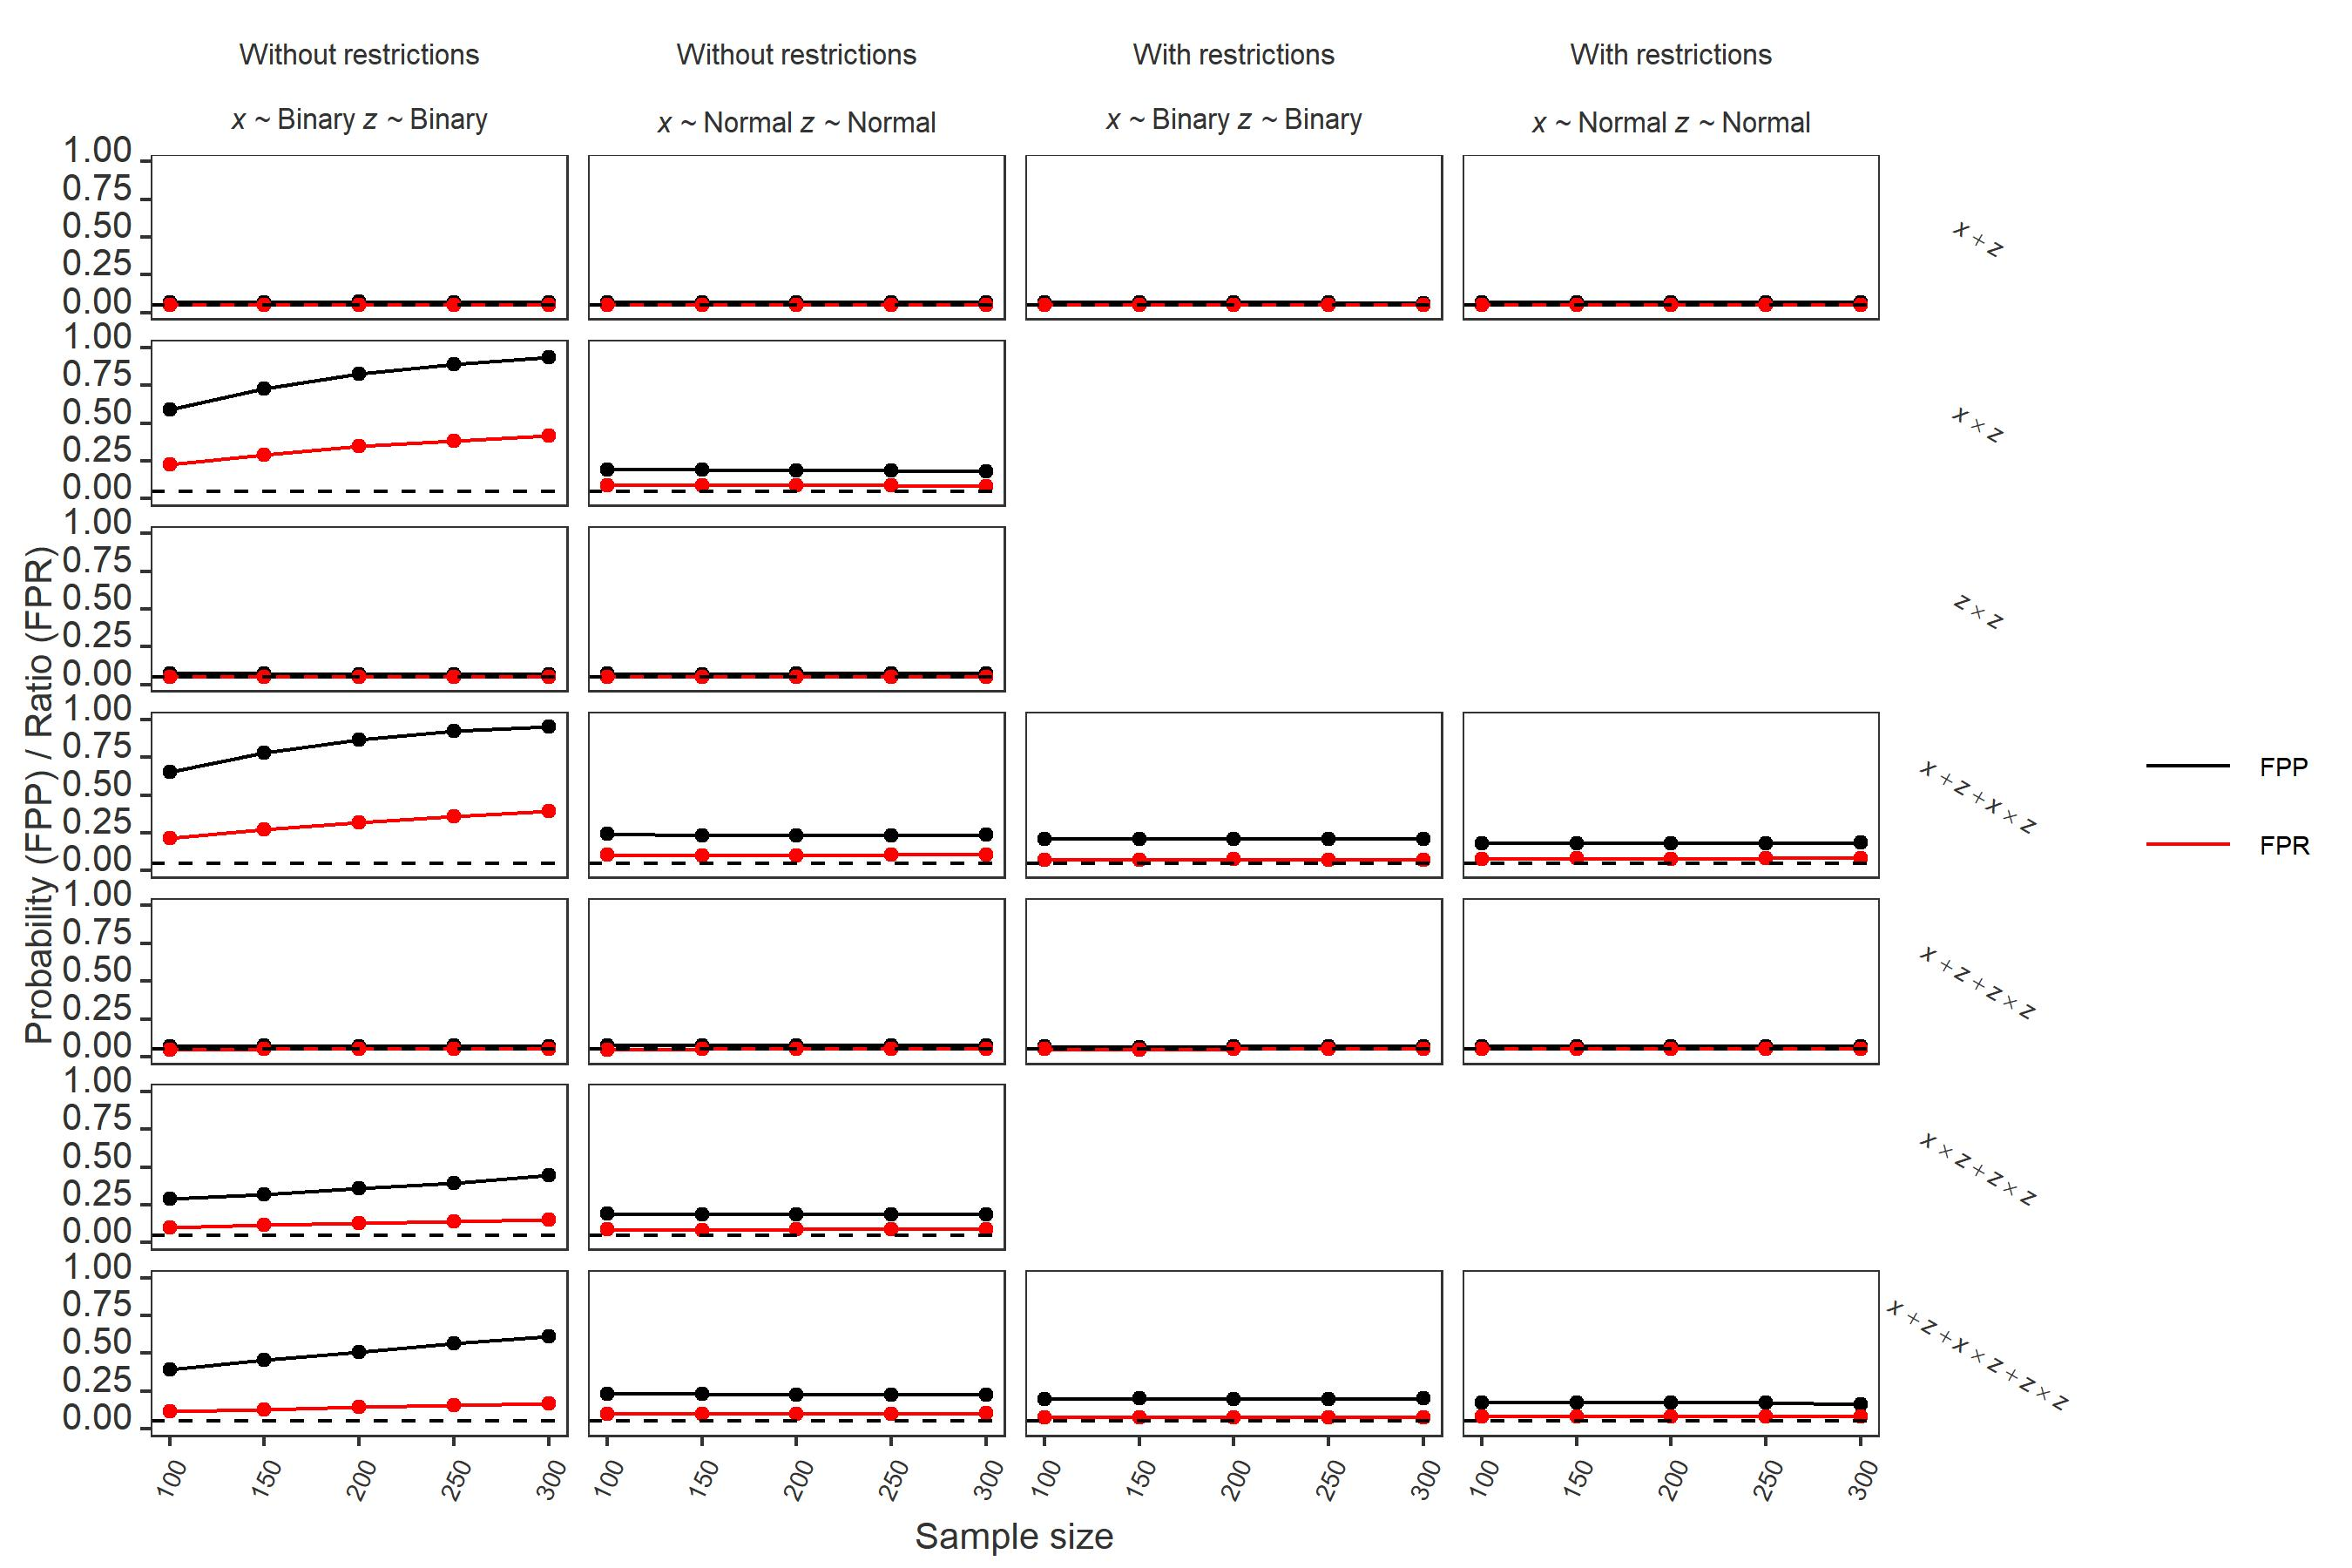
\includegraphics[width=0.9\textwidth]{R/Analysis/Result/Figures/Figure1D.jpeg}
\centering
\caption{The effect of increasing sample size on the false-positive probability and false-positive ratio. Black denotes the false-positive probability and red denotes the false-positive ratio. Dashed blacked line shows the critical value, here set at 0.05. The description of the figure is otherwise the same as for Figure \ref{fig:mainfigure1}.}
\label{fig:mainfigure4}
\end{figure}

\subsection{Correlation between dependent variable and covariates}
Increasing the correlation between the dependent variable and  covariates in the baseline model increases the FPP for most conditions and the FPR for some conditions (see Figure \ref{fig:appfigure1app}). The model sets with interactions between the variable of interest and covariates have the highest increase in both the FPP and FPR. The effect is most pronounced when the variable of interest and covariates are binary and dummy coded. The increase in the FPP for these sets is as high as 26.5 percentage points when the correlation increases from $r=0.2$ to $r=0.3$. When the correlation increases from $r=0.3$ to $r=0.4$, the FPP increases only in some conditions where the FPP is not already close to 100\%. The increase in correlation also affects the FPR for the same sets increasing it to as much as 14.4\% when going from $r=0.2$ to $r=0.3$ and similarly when going from $r=0.3$ to $r=0.4$. This increase is however not only present when there is allowed for interactions without main effects. Even in the correct specified models the FPP increases to some extent when there is an increase in the correlation between the dependent variable and the covariates. As in the misspecified models this happens when there are interactions between the variable of interest and the covariates. 